Seit der Entdeckung der kosmischen Höhenstrahlung
1912 von Victor Hess feiert die Astroteilchenphysik bahnbrechende Errungenschaften.
Die Entdeckung der kosmischen Hintergrundstrahlung gilt als Beleg des
expandierenden Universums und wirft dennoch weitere Fragen zum frühen Universum auf.
Die Kosmische Strahlung lässt das erforschen elementarer Bausteine und
Beschleunigungsprozesse zu,
wovon einige Informationen über ihren Ursprung tragen.
Anhand der kosmischen Botenteilchen, zu denen neuerdings auch Gravitationswellen
zählen, werden Informationen über Supernovae, Schwarze Löcher und Aktive
Galaxienkerne extrahiert.

\section*{MAGIC}%
\label{sec:magic}

\begin{wrapfigure}[13]{o}{0.45\textwidth}
		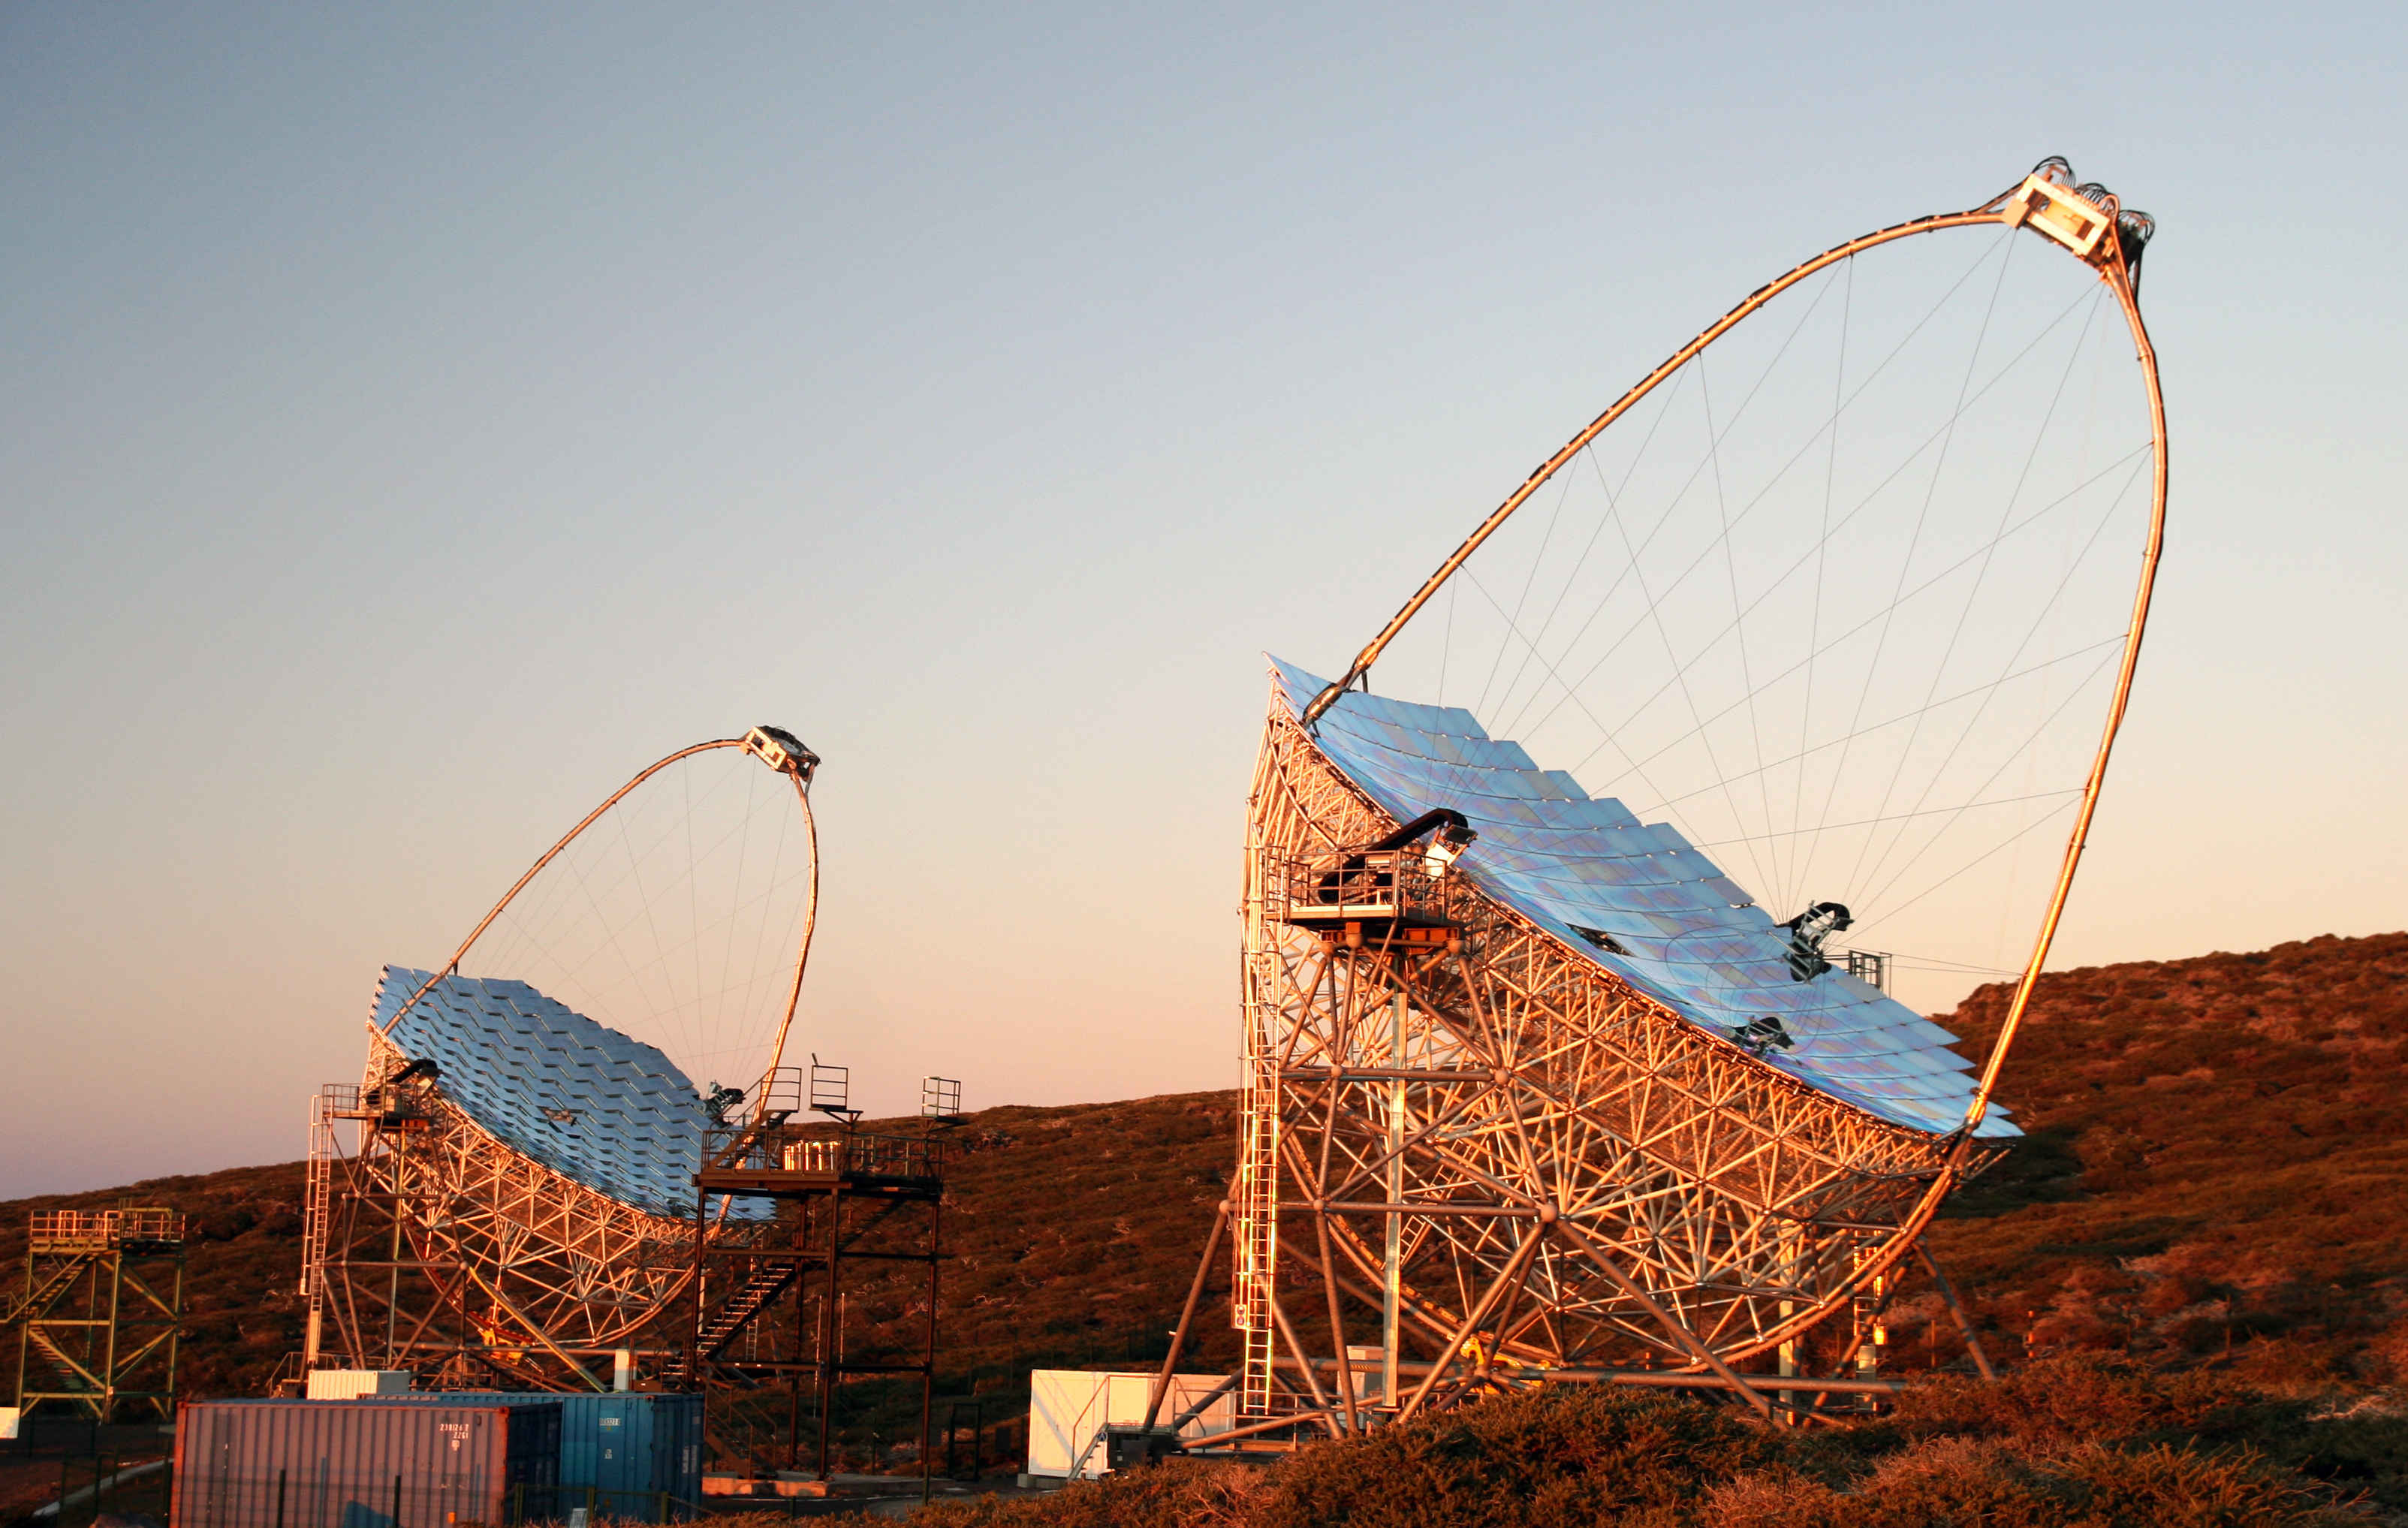
\includegraphics[width=\linewidth]{pictures/magic.JPG}
		\caption{MAGIC Teleskope in Observationsstellung.}%
		\label{fig:magic}
\end{wrapfigure}

Der Nachweis von hochenergetischer Gammastrahlung ist auf der Erde aufgrund der
Atmosphäre nur indirekt möglich.
Hochenergetische Teilchen erzeugen in der Atmosphäre Teilchenschauer, die
aufgrund ihrer relativistischen Geschwindigkeiten Tscherenkowlicht abstrahlen.
MAGIC ist derzeit (16.11.2016) das größte Stereoteleskop, mit dem die
Detektion von Tscherenkowschauern in einem Energiebereich von
\SI{50}{\giga\electronvolt} bis \SI{50}{\tera\electronvolt} möglich ist.
Es steht auf der Insel La Palma auf einer Höhe von \SI{2200}{\meter}.
Propagiert ein Teilchen mit einer Geschwindigkeit in einem Medium, die höher
ist, als die Lichtgeschwindigkeit in diesem Medium, so emittiert
es einen Tscherenkowkegel.
Die ultrarelativistischen Teilchen, welche auf die Erdatmosphäre treffen,
wechselwirken mit den darin enthaltenen Teilchen beispielsweise über
Bremsstrahlung oder Paarerzeugung und produzieren somit weitere
relativistische Teilchen, welche wiederum Tscherenkowkegel erzeugen.

Die dadurch erzeugten Lichtblitze können durch Tscherenkowteleskope detektiert
werden.
Die Spiegelfläche von \SI{17}{\meter} Durchmesser besteht aus \num{974} einzelnen
Spiegeln, die auf \num{1039} Photo Multiplier Tubes (PMTs) mit einem
Field of View von \SI{3.5}{\degree} abbilden.

Ziel ist es, mit den Teleskopen Gamma-Quellen wie AGNs, Supernovae und
Gasverteilungen, in denen viel Sternbildung stattfindet, genauer zu observieren.
Des Weiteren wird nach einen indirekten Nachweis nach dunkler Materie gesucht.
Fundamentales Problem ist, dass geladene Teilchen jegliche Richtungsinformation
in kosmologischen Magnetfeldern verlieren und somit keine Informationen zur
Quelle rekonstruiert werden kann.

\section*{Krebsnebel}%
\label{sec:krebsnebel}

In diesem Versuch wird der Krebsnebel untersucht.
Er ist ein Überrest einer Supernova-Explosion eines Sterns
mit 8~bis 12 Sonnenmassen aus dem Jahre 1054,
und befindet sich im Sternbild Stier.

\begin{wrapfigure}[16]{L}{0.35\textwidth}
		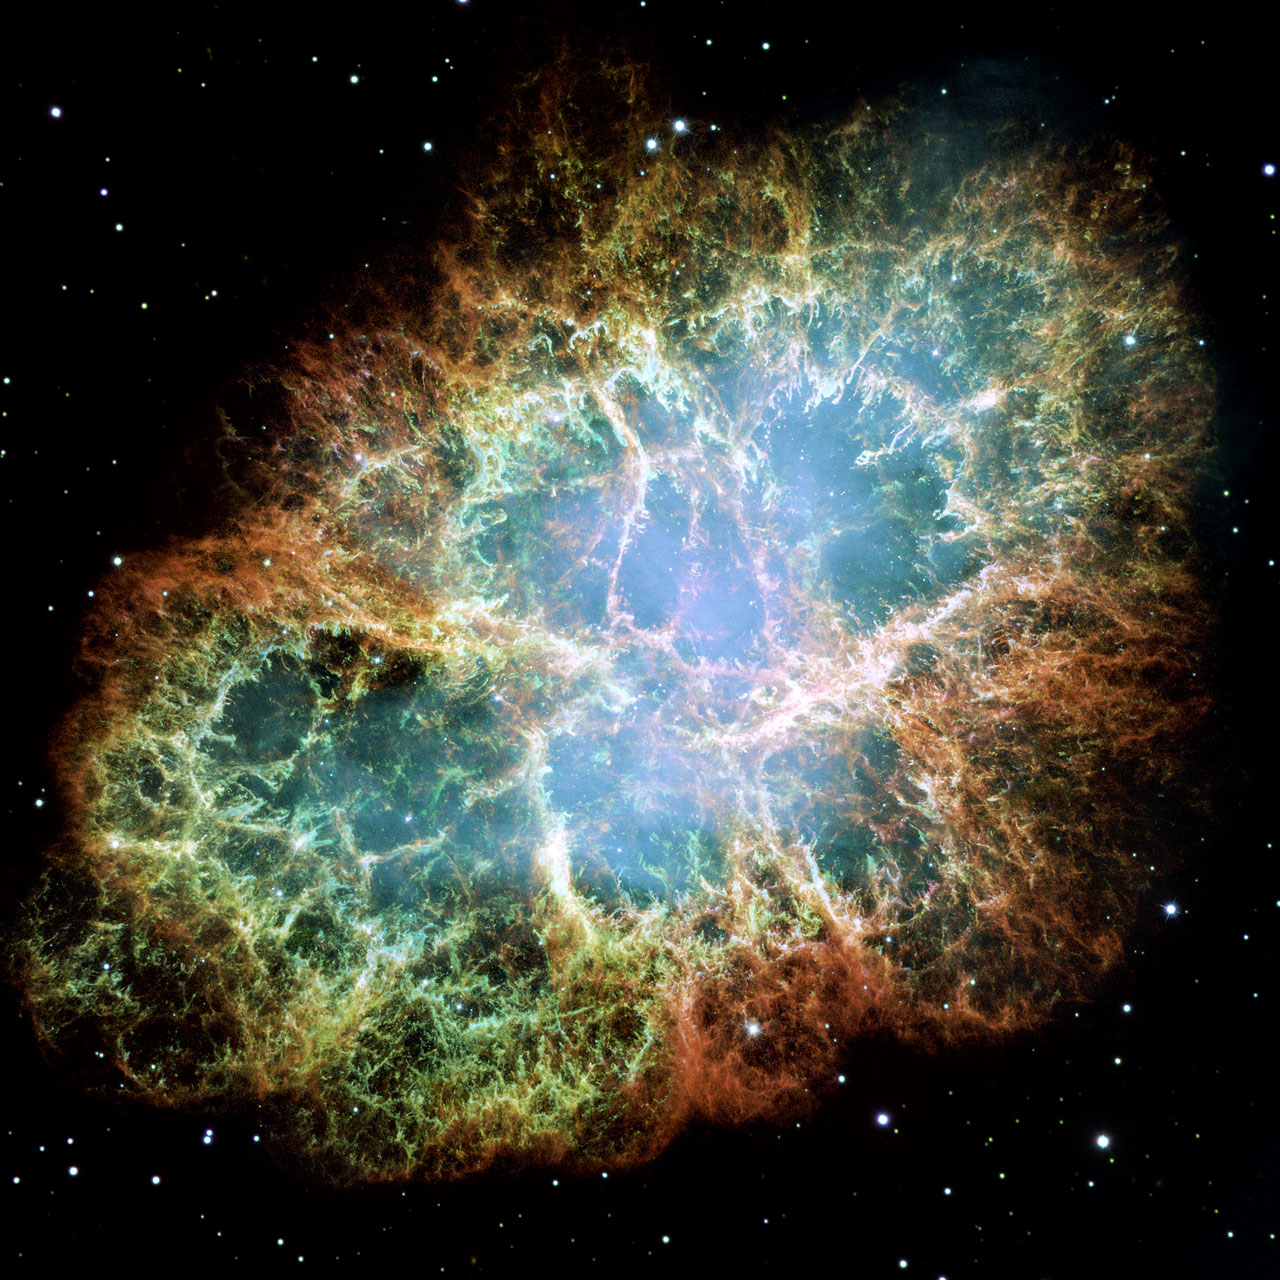
\includegraphics[width=\linewidth]{pictures/crab.jpg}
		\caption{Krebsnebel aufgenommen mit dem Hubble Teleskop.}%
		\label{fig:magic}
\end{wrapfigure}

Eine Supernova-Explosion ist das Ende eines massereichen Sterns,
welcher jedoch nicht schwer genug
für die Bildung eines schwarzen Loches ist.

Im Zentrum befindet sich ein Pulsar, welcher die Quelle von starker
elektromagnetischer Strahlung ist.
Pulsare sind schnell rotierende Neutronensterne,
welche sehr regelmäßige, kurze Pulse emittieren.
Typische Größen von Neutronensternen sind Durchmesser von einigen
\SI{10}{\kilo\meter}.
Die Materiereste, die bei einer Supernova-Explosion
vom zurückbleibenden Neutronenstern abgesprengt werden,
bilden eine Astronomisches Objekt,
welches sich in Astronomischen Zeitskalen schnell verändert.

Der Krebsnebel kann in allen Kanälen von der Radioastronomie bis hin zur Gammaastronomie observiert werden.
Aufgrund seiner Eigenschaften wird er als Standardkerze der Astronomie betitelt,
da die Eigenschaften sehr gut bekannt sind.
Durch seine Analyse kann die Performance von verschiedenen Teleskopen verglichen werden.
\clearpage
